% ----------------------------------------------------------
% Teste test1_1_e5b32class10_20231211_214334
% ----------------------------------------------------------
\subsubsection{Teste test1_1_e5b32class10_20231211_214334 - AlexNet (Is That a Santa)}

Informações utilizadas para o treinamento.

\begin{table}[ht]
   \centering
   \caption{Treinamento}
   \label{tab:modelos}
   \begin{tabular}{| c | c | }
      \hline 
      \textbf{Informação} & \textbf{Descrição} \\
      \hline \hline 
      Rede & AlexNet \\
      \hline
      Número de épocas & 5\\
      \hline
      Tamanho do lote & 32\\
      \hline
      Taxa inicial & 0.01 \\
      \hline
      Taxa de decaimento & 0.0005 \\
      \hline
      Total de classes & 10\\
      \hline
      Dataset & CIFAR-10\\
      \hline
   \end{tabular} 
\end{table}

Resultados obtidos após treinamento.

\begin{tabular}{lrrrr}
\toprule
  Unnamed: 0 &  precision &  recall &  f1-score &    support \\
\midrule
    airplane &   0.855866 &  0.7660 &  0.808443 &  1000.0000 \\
  automobile &   0.947368 &  0.8100 &  0.873315 &  1000.0000 \\
        bird &   0.663826 &  0.7010 &  0.681907 &  1000.0000 \\
         cat &   0.593269 &  0.6170 &  0.604902 &  1000.0000 \\
        deer &   0.754386 &  0.7310 &  0.742509 &  1000.0000 \\
         dog &   0.732955 &  0.6450 &  0.686170 &  1000.0000 \\
        frog &   0.748722 &  0.8790 &  0.808648 &  1000.0000 \\
       horse &   0.772251 &  0.8850 &  0.824790 &  1000.0000 \\
        ship &   0.896951 &  0.8530 &  0.874423 &  1000.0000 \\
       truck &   0.831721 &  0.8600 &  0.845624 &  1000.0000 \\
    accuracy &   0.774700 &  0.7747 &  0.774700 &     0.7747 \\
   macro avg &   0.779732 &  0.7747 &  0.775073 & 10000.0000 \\
weighted avg &   0.779732 &  0.7747 &  0.775073 & 10000.0000 \\
\bottomrule
\end{tabular}


\begin{figure}[ht]
 \begin{center}
   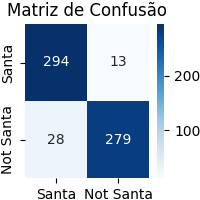
\includegraphics[scale=1]{tests/test1_1_e5b32class10_20231211_214334/confusion_matrix.png}
  \caption{Matriz de Confusão}
  \label{fig:fig03}
 \end{center}
\end{figure}

\begin{figure}[ht]
 \begin{center}
   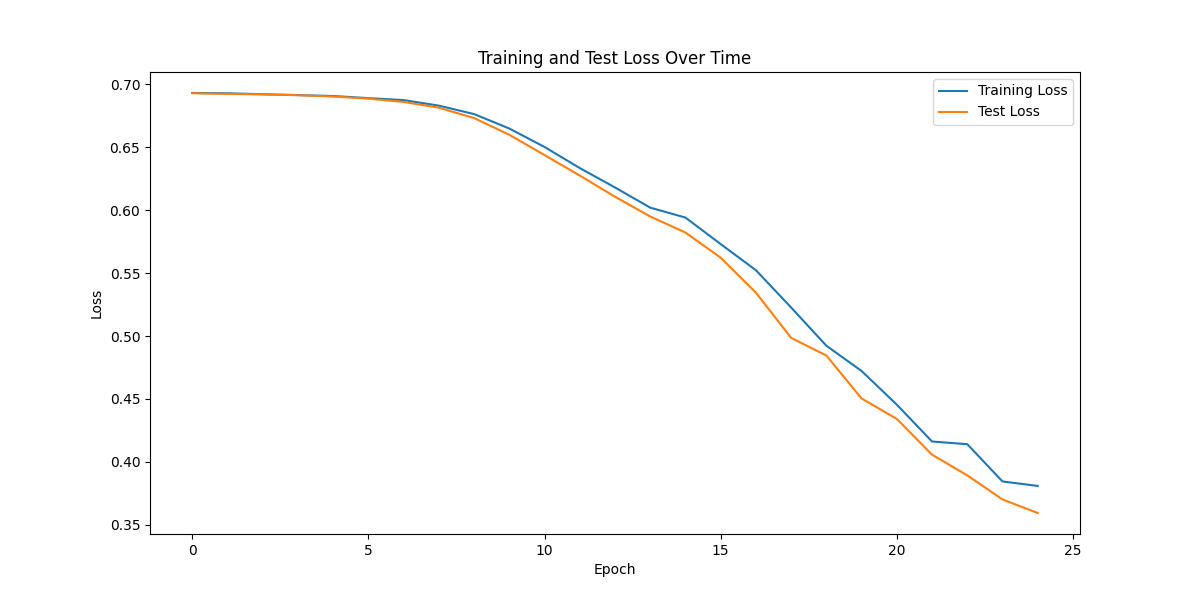
\includegraphics[scale=0.8]{tests/test1_1_e5b32class10_20231211_214334/loss_over_time.png}
  \caption{Gráfico de Perda}
  \label{fig:fig04}
 \end{center}
\end{figure}
